\chapter{Экспериментальная часть}

В данном разделе будет произведено сравнение вышеизложенных алгоритмов.

\section{Временные характеристики}

Для сравнения возьмем изображение размером 1200$\times$700.
Так как трассировка данного изображения считается достаточно короткой
задачей, воспользуемся усреднением массового эксперимента.
Сравнение произведем при n = 50.

Результат представлен на рис.  \ref{ref:time}.

\begin{figure}[ht!]
	\centering{
		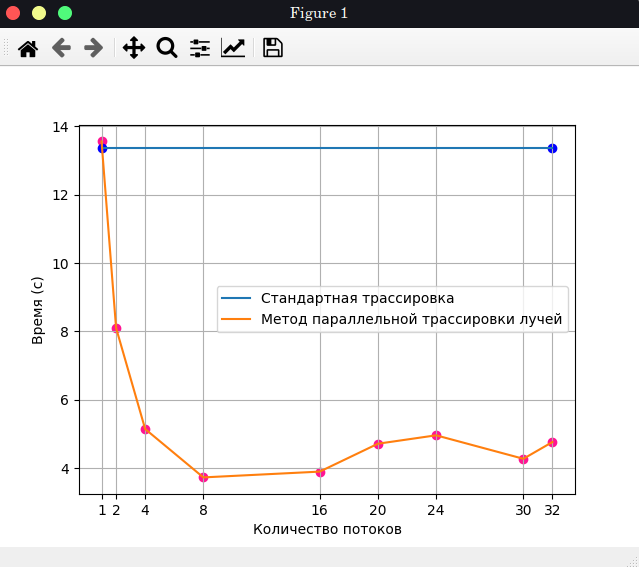
\includegraphics[width=0.8\textwidth]{time.png}
		\caption{Временные характеристики}
		\label{ref:time}}
\end{figure}


Обычная реализация работает быстрее, чем создание одного потока,
потому что на создание потока тратится некоторое время.
При двух потоках выигрыш получается почти в два раза, так как два потока
трассируют одновременно свою часть экрана.
При увеличении числа потоков отслеживается уменьшение времени трассировки.
При 8 потоках достигается пик, при котором все ядра процессора одновременно
выполняют трассировку экрана.
Далее при увеличении числа потоков производительность падает.
Это объясняется тем, что создается очередь потоков, которая замедляет
работу программы.

\section{Вывод}

В данном разделе было произведено сравнение алгоритма трассировки лучей
при простой реализации и многопоточной (рис. \ref{ref:time}). Результат показал, что
выгоднее всего использовать все ядра процессора.